\documentclass[12pt]{article}

% Style
\usepackage{parskip}	% Blank line between paragraphs
\usepackage[top=1in, bottom=1.25in, left=1.25in, right=1.25in]{geometry} % Page margins
\usepackage{float} % Placement of figures with H
\renewcommand{\familydefault}{\sfdefault} % Use sans-serif font (https://tex.stackexchange.com/a/2097)

% Maths
\usepackage{graphicx}
\usepackage{amsmath}
\usepackage{amssymb}
\usepackage{units}

\usepackage[hidelinks, pdfusetitle]{hyperref}

% Code listings, https://tex.stackexchange.com/a/99476
\usepackage{minted}
\usemintedstyle{vs}

% Utillities
\usepackage{framed}   % Draw frames around paragraphs
\usepackage{listings} % Code listings
\usepackage{color}
\usepackage{array}

% Settings
\allowdisplaybreaks		% Break aligned equations over pages

\usepackage{perpage}      % Reset footnote counter per page (1)
\MakePerPage{footnote}    % Reset footnote counter per page (2)

% Change itemize label items
\renewcommand{\labelitemi}{$\bullet$}
\renewcommand{\labelitemii}{$\bullet$}
\renewcommand{\labelitemiii}{$\bullet$}

% Parameters
\newcommand{\version}{0.7}
\newcommand{\website}{\href{http://www.virtualbow.org/}{\texttt{\textcolor{blue}{http://www.virtualbow.org/}}}}
\newcommand{\copyrights}{Copyright (C) 2016-2020 Stefan Pfeifer}

\begin{document}

\begin{titlepage}

\vspace*{5em}
\centering{\Huge\textbf{VirtualBow~v\version \\[1em] User Manual}}

\vspace{5em}

\centerline{
\includegraphics[width=0.2\textwidth]{figures/logo.pdf}}

\null
\vfill
\centerline{\copyrights}

\thispagestyle{empty}
\end{titlepage}

\newpage
\tableofcontents

\newpage
\section{Introduction}
\bigskip

VirtualBow is a software tool for bow and arrow physics simulation.
It allows you to design virtual bow models, simulate their static and dynamic behaviour and visualize the results, providing almost immediate feedback about the bow's predicted performance.
The application consists of the following three components:

\begin{itemize}
\item \textbf{VirtualBow:} The model editor and core of the application.
Create, load and save bow models (.bow), edit their various parameters and launch static and dynamic simulations.
The model editor takes care of calling the other two components, VirtualBow Solver and VirtualBow Post, although those can be used independently as well.

\item \textbf{VirtualBow Post:} This is the result viewer. It is used for opening and visualizing the simulation results (.res) produced by the solver.
Here you can analyze and evaluate your bow designs.

\item \textbf{VirtualBow Solver:} The solver performs the actual simulation. It takes a model file (.bow), does the necessary numerical calculations and writes a result file (.res) that can be opened with the result viewer or analyzed by other programs.
\end{itemize}

\bigskip

The following chapters of this manual will show you how to use the software and its components and explain the various input parameters and simulation results. For help and support, giving feedback or to get the latest version of the software and this manual please visit the project's website at \website

\newpage
\section{VirtualBow}

\subsection{Overview}

This is the main application.
Here you can load, edit and save bow models and launch simulations.

\begin{figure}[H]
\centering
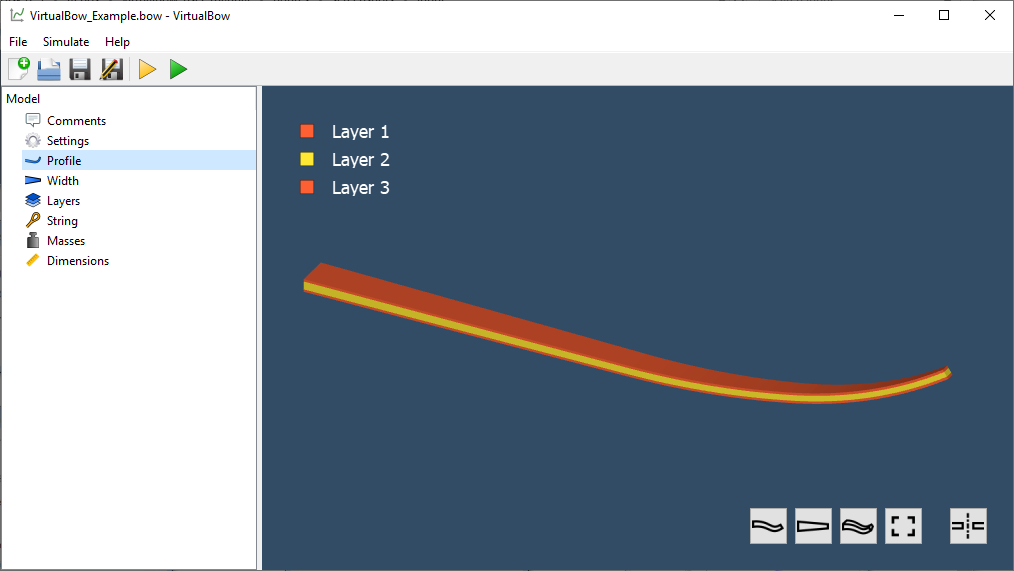
\includegraphics[width=\textwidth]{figures/screenshots/input/bow-editor}
\caption{Bow Editor}
\label{fig:bow-editor}
\end{figure}

All the parameters of the bow can be accessed via the model tree on the left.
Double-click any of the items to edit the respective category.
The next sections will cover each of those items in more detail.

The 3D view on the right shows the bow's current geometry resulting from those parameters.
Use the mouse to rotate (left button), shift (middle button) and zoom (mouse wheel).
More options are available through the buttons on the bottom-right corner.

Use the main menu and/or the toolbar to create, load and save bow models, which are stored as .bow files.
Run a static simulation to analyze the bow being drawn or a dynamic simulation to analyze the bow in motion, i.e. when shooting an arrow.
The simulation results will be stored next to the model file and opened in VirtualBow Post.

\newpage
\subsection{Parameters}

\subsubsection{Comments}

The comments are meant for documenting the bow model.
Any notes about the bow, its paramters or the simulation results can be added here.
\bigskip

\begin{figure}[H]
\centering
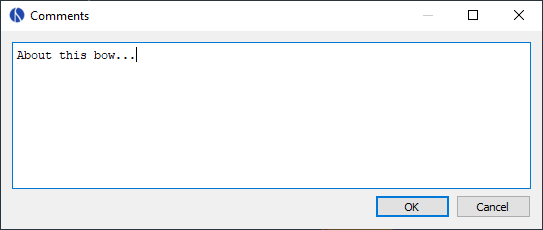
\includegraphics[width=0.7\textwidth]{figures/screenshots/input/comments}
\caption{Comments dialog}
\label{fig:comments}
\end{figure}

\subsubsection{Settings}

These are numerical settings that can be used to tweak the simulation.
Most of the time the default values should be fine though, so if you're reading this manual for the first time you might want to skip this section.

\bigskip

\begin{figure}[H]
\centering

\includegraphics[width=0.4\textwidth]{figures/screenshots/input/settings}
\caption{Settings dialog}
\label{fig:settings}
\end{figure}

\newpage

Since the default settings are meant to be a good general choice, they favor accuracy and reliability over simulation performance.
So for specific use cases it might be an advantage to find more efficient settings.
Think about running a large number of scripted simulations, for example.
On the other hand, even the default settings might sometimes fail with certain bow designs such that different settings have to be used.

\paragraph*{General}

\begin{itemize}
\item \textbf{Limb elements:} Number of finite elements that are used to approximate the limb. More elements increase the accuracy but also the computing time.
\item \textbf{String elements:} Number of finite elements that approximate the string. This number can usually be reduced if the bow has no recurve. In the case of a static analysis with no recurve it can even be set to one without losing any accuracy.
\end{itemize}

\paragraph*{Statics}

\begin{itemize}
\item \textbf{Draw steps:} Number of steps that are performed by the static simulation from brace height to full draw. This determines the resolution of the static results. You can usually decrease this value to speed up the simulation, especially if you're only interested in the dynamic results.
\end{itemize}

\paragraph*{Dynamics}

\begin{itemize}
\item \textbf{Time span factor:} This controls the time period that is simulated. A value of $1$ corresponds to the time at which the arrow passes the brace height. The default value is larger than that in order to capture some of the things that occur after the arrow left the bow (maximum dynamic loads on limb and string).
\item \textbf{Time step factor:} When simulating the dynamics of the bow, the program will repeatedly use the current state of the bow at time $t$ to calculate the next state at time $t + \Delta t$ where $\Delta t$ is some small timestep. We want this timestep to be as large as possible to keep the computational cost low. But it still has to be small enough to get an accurate and stable solution. The program will estimate this optimal timestep, but to be on the safe side the estimation is multiplied with a reduction factor between $0$ and $1$ that you can choose here.
\item \textbf{Sampling rate:} The sampling rate limits the time resolution of the output data. This is done because the dynamic simulation usually produces much finer grained data than is actually useful. Not including all of that in the final output reduces simulation time and memory consumption.
\end{itemize}

\newpage
\subsubsection{Dimensions}
\label{sec:dimensions}

The parameters listed in this dialog define the overall lengths and angles of the bow and its optional stiff middle section. See figure~\ref{fig:dimensions-2} for a visual explanation of those.
\bigskip

\begin{figure}[H]
\centering
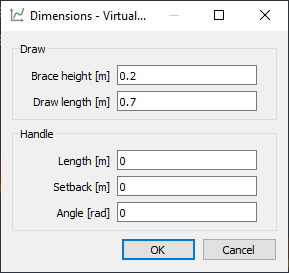
\includegraphics[width=0.4\textwidth]{figures/screenshots/input/dimensions}
\caption{Dimensions dialog}
\label{fig:dimensions-1}
\end{figure}

\begin{figure}[H]
\centering
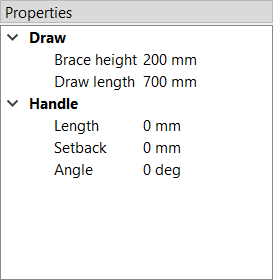
\includegraphics[width=0.4\textwidth]{figures/dimensions}
\caption{Dimensions of the bow}
\label{fig:dimensions-2}
\end{figure}

\newpage
\subsubsection{Profile}

The profile curve is the geometric centerline of the bow's limbs in unbraced state.
Edit the parameters in the table on the left and view the resulting profile curve on the plot on the right.

\bigskip

\begin{figure}[H]
\centering
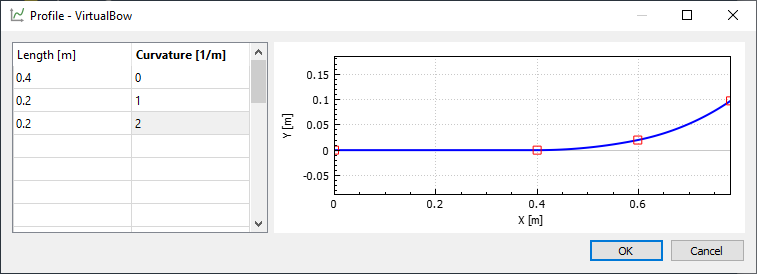
\includegraphics[width=\textwidth]{figures/screenshots/input/profile}
\caption{Profile dialog}
\label{fig:profile}
\end{figure}

The profile curve is defined by a series of points where each point has an arc length and a curvature.
The arc length is the distance of the point along the curve.
Because of that, the last point also defines the total length of the profile curve.
The curvature is interpolated linearly between the points, which ensures that there are no jumps in curvature, only smooth transitions.

\bigskip

\textbf{Note:} The profile curve always starts at (0, 0) and with a horizontal angle.
Any offsets can be achieved with the parameters under \textit{Dimensions}, see section \ref{sec:dimensions}.

\bigskip

\textbf{Note:} Two points with zero curvature produce a straight line segment while two points with equal and non-zero curvatures produce a circular segment. Two points with different curvatures produce a spiral segment\footnote{\url{https://en.wikipedia.org/wiki/Euler_spiral}} that transitions between the two curvatures.

\bigskip

\textbf{Note:} Mathematically, the curvature $\kappa$ of a curve is the inverse of its radius of curvature $r$, so you can calculate the curvature via $\kappa = \nicefrac{1}{r}$ if you know the radius at that point and vice versa.

\newpage
\subsubsection{Width}

The width dialog is used to define the limb's width along its profile curve. This width is the same for all layers of the bow.

\bigskip

\begin{figure}[H]
\centering

\includegraphics[width=\textwidth]{figures/screenshots/input/width}
\caption{Width dialog}
\label{fig:width}
\end{figure}

On the table on the left you can specify values for the width at certain relative positions (between 0 and 1) along the limb. This definition of cross section properties relative to the total length of the limb makes it possible to later change the profile curve without having to adjust any cross sections.

The actual width distribution of the limb is constructed as a smooth curve (monotonic cubic spline) passing through the supplied values as shown on the plot on the right.

\newpage
\subsubsection{Layers}

With the layer dialog you can create any number of layers and specify their height/thickness and material properties.
\bigskip

\begin{figure}[H]
\centering

\includegraphics[width=\textwidth]{figures/screenshots/input/layers}
\caption{Layer dialog}
\label{fig:width}
\end{figure}

Click the plus button on the top left to add layers or delete them by closing their tab.
Rearrange the order of the layers by dragging the tabs.
Double-click on a tab to rename a layer.

The table on the left sets the height distribution of the layer. It works the same way as the limb's width: You specify a number of values at different relative positions, which the program uses to create an interpolating curve. (In this case also a monotonic cubic spline.)

The layer's material is specified by the following two constants,

\begin{itemize}
\item \textbf{rho:} Density (Mass per unit volume)
\item \textbf{E:} Elastic modulus (Measure for the stiffness of a material)
\end{itemize}

For synthetic materials like e.g. fiber-reinforced composites you can often find those numbers in a datasheet provided by the manufacturer.
Natural materials like wood are more difficult, because their properties can vary quite a bit.
You can find average numbers on the internet, for example at \url{http://www.wood-database.com}.
Those are probably good enough as a first reference.
However, in order to be really sure about a specific material there is no other way than to test it.
One possibility is a simple bending test as shown in Appendix~\ref{sec:bending-test}.

\newpage
\subsubsection{String}

Here you can define the mechanical properties of the string by providing data for the string material and the number of strands being used.

\bigskip

\begin{figure}[H]
\centering
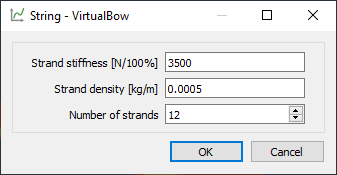
\includegraphics[width=0.4\textwidth]{figures/screenshots/input/string}
\caption{String dialog}
\label{fig:string}
\end{figure}

\begin{itemize}
\item \textbf{Strand density:} Linear density of the strands (mass per unit length)
\item \textbf{Strand stiffness:} Stiffness of the strands against elongation (force per unit strain)
\item \textbf{Number of strands:} Total number of strands in the string
\end{itemize}

\bigskip

\textbf{Note:} The stiffness of the string material can be an important parameter in dynamic analysis.
The static results however aren't affected very much by it as long as the value is high enough to prevent significant elongation.

\textbf{Note:} The linear density of a string material can be easily determined with a kitchen scale (weight divided by length).
The stiffness however is much more difficult to obtain.
Manufacturers of string materials usually don't publish those numbers.
Table~\ref{tbl:string-materials} shows the results of tensile tests for three common bow string materials.
They were done by the German Institutes for Textile and Fiber Research\footnote{\url{https://www.ditf.de/en/index/ditf.html}} in July 2018.

\bigskip

\begin{table}[H]
\centering
\begin{tabular}{ | p{75pt} | p{70pt} | p{70pt} | p{80pt} | p{90pt} | }
\hline
\textbf{Material} & \textbf{Density} [\unitfrac{kg}{m}] & \textbf{Breaking strength} [\unit{N}] & \textbf{Elongation at break} [\unit{\%}] & \textbf{Stiffness (linearized)} [\unitfrac{N}{100\%}] \\ \hline
Dacron B50      & 370e-6 & 180 & 8.5 & 2118 \\ \hline
Fastflight Plus & 176e-6 & 318 & 2.9 & 10966 \\ \hline
BCY 452X        & 192e-6 & 309 & 2.5 & 12360 \\ \hline
\end{tabular}
\caption{Test results for some common bowstring materials, the stiffness was estimated from breaking strength and elongation}
\label{tbl:string-materials}
\end{table}

\newpage
\subsubsection{Masses}

This dialog is used to define various individual masses of the bow.
Only the mass of the arrow is actually required, the other ones are optional and may also be set to zero.

\bigskip

\begin{figure}[H]
\centering
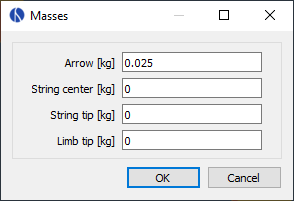
\includegraphics[width=0.4\textwidth]{figures/screenshots/input/masses}
\caption{Masses dialog}
\label{fig:masses}
\end{figure}

\begin{itemize}
\item \textbf{Arrow:} Mass of the arrow
\item \textbf{String center:} Additional mass at the string center (serving, nocking point)
\item \textbf{String tip:} Additional mass at the ends of the string (serving, silencers)
\item \textbf{Limb tip:} Additional mass at the limb tip (nocks, overlays)
\end{itemize}

\newpage
\subsubsection{Damping}

This dialog allows setting a damping ratio for the limbs and string, respectively.
Those parameters can be used to adjust for the energy a bow loses by dissipation, for example due to internal friction/hysteresis of the materials.

\bigskip

\begin{figure}[H]
\centering

\includegraphics[width=0.4\textwidth]{figures/screenshots/input/damping}
\caption{Damping dialog}
\label{fig:damping}
\end{figure}

\textbf{Note:} The damping ratio characterizes how quickly oscillations in a system decay over time.
A system with a damping ratio of 0\% is undamped, it doesn't dissipate any energy and just keeps going with a constant amplitude.
The higher the damping ratio the faster the amplitudes decay over time, losing energy with each oscillation.
Once the damping ratio reaches 100\% the system no longer oscillates at all (no overshoot), this is called critical damping.

\begin{table}[H]
\centering
\begin{tabular}{| m{4cm} | m{4cm} |}
\hline
\textbf{Damping ratio} & \textbf{Amplitude} \\ \hline
\center 0\% & 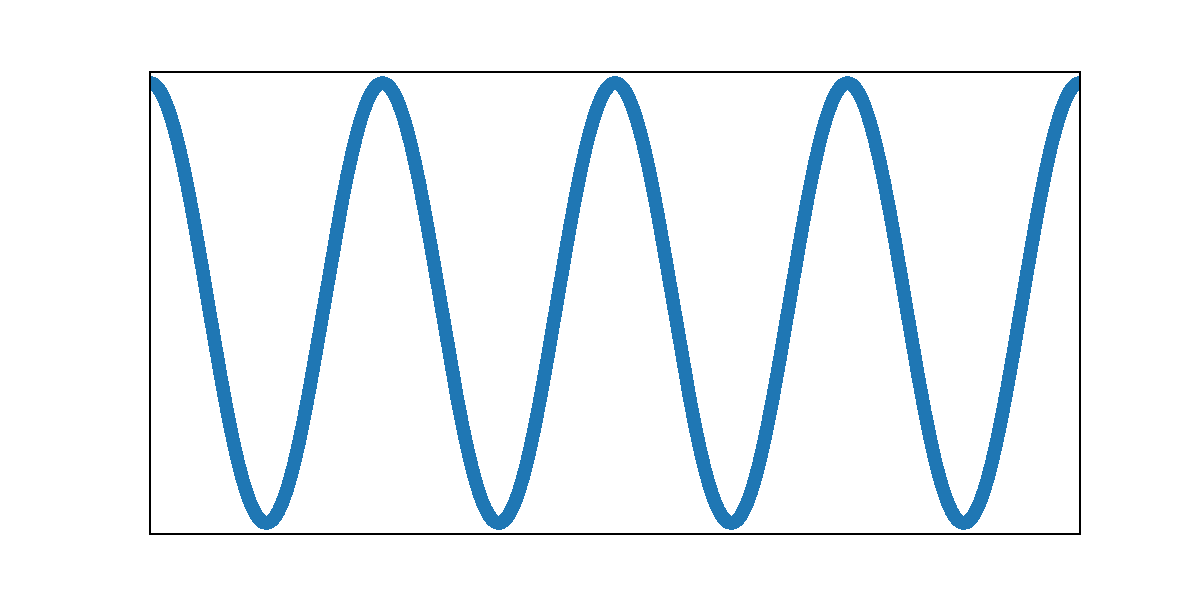
\includegraphics[width=0.25\textwidth]{figures/damping-ratio-00} \\ \hline
\center 10\% & 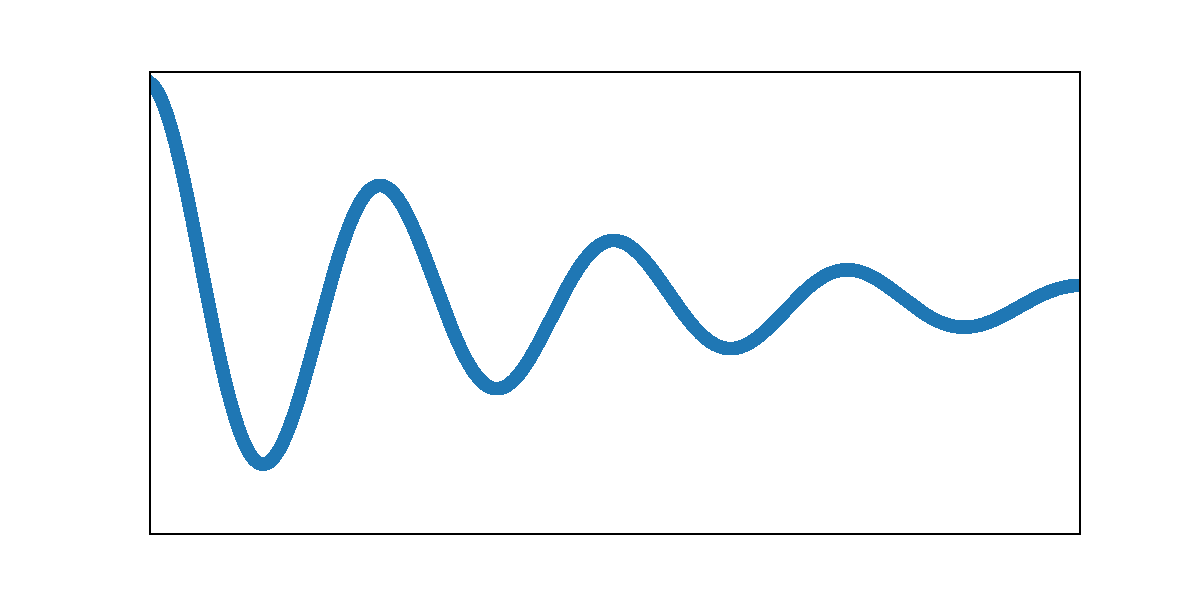
\includegraphics[width=0.25\textwidth]{figures/damping-ratio-01} \\ \hline
\center 100\% & 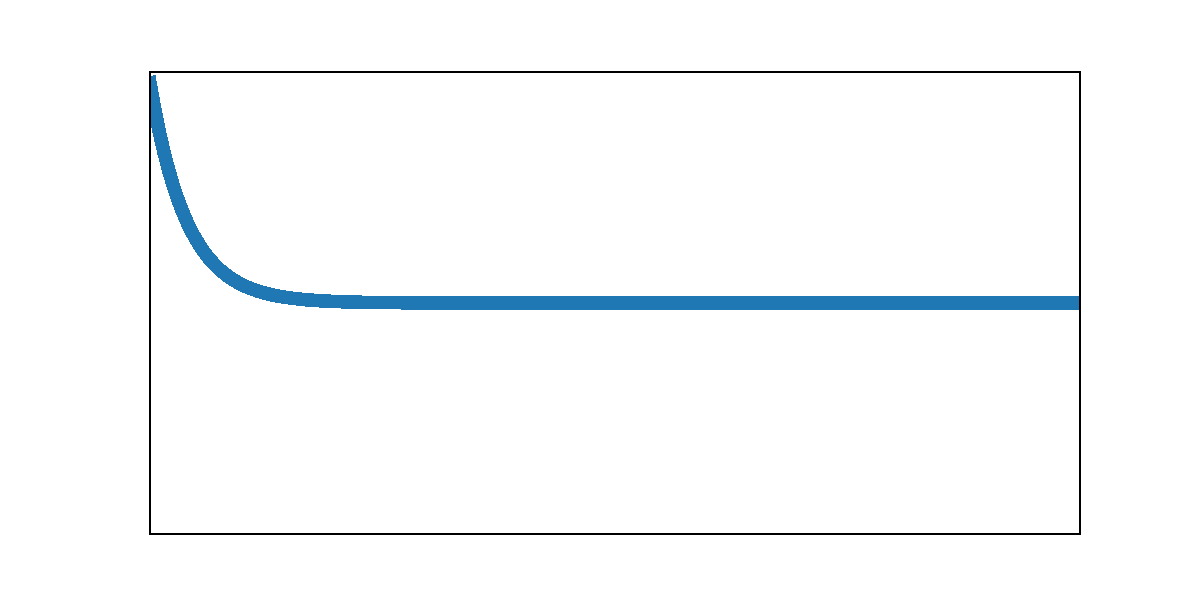
\includegraphics[width=0.25\textwidth]{figures/damping-ratio-10} \\ \hline
\end{tabular}
\caption{Oscillations with increasing damping ratio}
\label{tbl:damping-ratio}
\end{table}

The damping ratios for a bow's limbs and string are mostly empirical and there isn't yet any practical experience with those parameters in VirtualBow.
Realistic values are probably in the range of 0 - 20\% though.



\newpage
\section{VirtualBow Post}

\subsection{Overview}

This part of the application is used to open and visualize simulation results that are stored in .res files.
It is launched automatically by the model viewer when a simulation has finished, but it can also be used as a standalone application.
\bigskip

\begin{figure}[H]
\centering
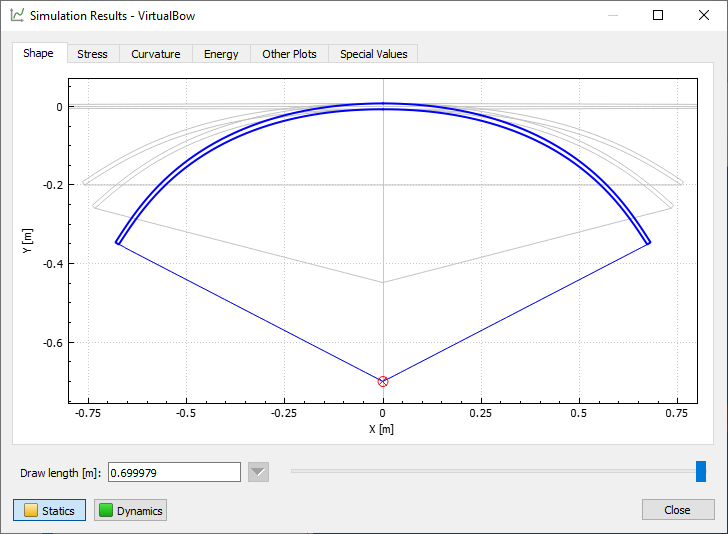
\includegraphics[width=\textwidth]{figures/screenshots/output/result-window}
\caption{Simulation results}
\label{fig:result-window}
\end{figure}

After loading a result file you can use the buttons on the bottom right corner of the window to switch between static and dynamic results, if available.
The results themselves are organized in different tabs, which will be explained in the next sections.

Below the tabs there is a slider where you can change the current state of the bow that is being viewed, either by draw length in the static case or by time in the dynamic case.
This value applies to all of the tabs.
Drag the slider to a specific position or use the play buttons to show the simulation results as a continuous animation.
The input field and the dropdown menu next to it allow you to jump directly to special points in the results, for example where certain forces or stresses reach their maximum or the arrow leaves the string. 

\newpage
\subsection{Results}

\subsubsection{Characteristics}

This tab shows all results that can be expressed as a single number.
Some of them differ between statics and dynamics.

\paragraph*{Statics}

\begin{itemize}
\item \textbf{Final draw force:} Draw force of the bow at full draw
\item \textbf{Drawing work:} Total work done by drawing the bow. This work is stored in the bow as potential elastic energy and later partially transfered to the arrow, depending on the bow's efficiency. It is equal to the area under the force-draw curve of the bow (See also \textit{Other Plots}).
    \item \textbf{Storage ratio:} This is an indicator of how much energy the bow stores and is defined as
$$\mathrm{storage\ ratio} = \frac{\mathrm{drawing\ work}}{1/2\cdot \mathrm{draw\ force}\cdot (\mathrm{draw\ length} - \mathrm{brace\ height})},$$
which is the amount of energy stored by the bow's draw curve in relation to a linear draw curve with the same final draw force.
\item \textbf{Limb mass:} Total mass of a single bow limb, including the additional tip mass
\item \textbf{String mass:}  Total mass of the bow string, including additional masses
\item \textbf{String length:} Length of the string, determined by the desired brace height
\end{itemize}

\paragraph*{Dynamics}

\begin{itemize}
\item \textbf{Final arrow velocity:} Velocity of the arrow when departing from the bow
\item \textbf{Degree of efficiency:} The bow's degree of efficiency, i.e. useful energy output (kinetic energy of the arrow) divided by energy input (static drawing work)
\item \textbf{Kinetic energy arrow:} Kinetic energy of the arrow on departure from the string
\item \textbf{Kinetic energy limbs:} Kinetic energy of the limbs on arrow departure
\item \textbf{Kinetic energy string:} Kinetic energy of the string on arrow departure
\end{itemize}

\paragraph*{Common}

\begin{itemize}
\item \textbf{Maximum absolute stresses:} Maximum stress by absolute value for each layer
\item \textbf{Maximum absolute forces:} Maximum forces by absolute value. Entries are the draw force, the string force and the grip support force, i.e. the force that is required to hold the bow handle at its position.
\end{itemize}

\subsubsection{Shape} Shows the shape of the limb and string as well as the position of the arrow at different stages of either the draw (statics) or the shot (dynamics).
The little red circle symbolizes the back end of the arrow.
You can use the slider at the bottom to change the current state of the bow or to view all states as a continuous animation.

\subsubsection{Stress} Shows the stress distribution along the limb for each one of the layers, evaluated at the back and belly sides.

\subsubsection{Curvature} Shows the curvature of the limb along its length.
This is not the total curvature but rather the difference to the unbraced shape.

\subsubsection{Energy} This plot shows how the total amount of energy in the bow develops during the simulation and how it is distributed between components (limbs, string arrow) and type of energy (potential/elastic or kinetic).
In the dynamic case it shows how the initial potential energy of the limbs is transferred to the arrow and other components of the bow and how much unused energy stays in the bow after the departure of the arrow.

\subsubsection{Other Plots} Here you can combine arbitrary simulation results and plot them together, e.g. things like the draw curve of the bow or the velocity of the arrow.

\newpage
\section{VirtualBow Solver}

\subsection{Command Line Interface}

The VirtualBow solver can be used from the command line to launch simulations in batch mode, without opening the GUI.
The executables for the three components of VirtualBow are named

\begin{framed}
\begin{verbatim}
virtualbow-gui        // Main program
virtualbow-slv        // Solver
virtualbow-post       // Result viewer
\end{verbatim}
\end{framed}

The solver command takes a model file as the input and produces a result file as the output.
The type of simulation (static or dynamic) as well as other options can be set.
The detailed usage as shown by the \texttt{--help} option is:

\bigskip

\begin{framed}
\begin{verbatim}
> virtualbow-slv --help
Usage: virtualbow-slv [options] input output

Options:
  -?, -h, --help  Displays this help.
  -v, --version   Displays version information.
  -s, --static    Run a static simulation.
  -d, --dynamic   Run a dynamic simulation.
  -p, --progress  Print simulation progress.

Arguments:
  input           Model file (.bow)
  output          Result file (.res)
\end{verbatim}
\end{framed}

\bigskip

\textbf{Note:} To use the command line interfaces on Windows you have to either specify the complete path to the respective executable or add the installation directory to your \texttt{PATH} environment variable.
There is an option to do this automatically during installation.

\bigskip

\textbf{Note:} On MacOS, the VirtualBow executables are hidden inside the application bundle.
They can be accessed by their full path though, or their location can be temporarily added to the PATH environment variable with the command

\begin{framed}
\begin{verbatim}
export PATH = $PATH:/Applications/VirtualBow.app/Contents/MacOS
\end{verbatim}
\end{framed}

Put this line into your \texttt{.bash\_profile} to make the change persistent.

\newpage
\subsection{Scripting}

The main use of the command line interface is the ability to write programs that automatically launch simulations and analyze their results.
This is especially useful when a large number of simulations has to be done, for example when performing design optimizations or exploring the influence of certain model parameters on the simulation results.
Launching simulations from the command line is only one part of this.
Scripts that interoperate with VirtualBow also have to be able to read and write the model and result files that constitute the input and output of the solver.

\textbf{Note:} Since VirtualBow is still far from finished, the contents of both of these files are subject to change.
The goal is to keep compatibility with older model files as much as possible, such that newer versions of VirtualBow can still open older files.
This might not always be possible though.
Any scripts that work with those files should therefore expect breaking changes in the future, which means that they will have to be updated in order to keep working with newer versions of VirtualBow.

\subsubsection*{Model Files}

The model files have a .bow extension, but are in fact just plain text JSON\footnote{\url{http://json.org}} files.
JSON is a very common human readable format for storing data in the form of objects, arrays, strings, numbers and more in a hierarchical way.
As the format is text based, it is possible to just open the model files with a text editor and have a look at contents.
For a detailed specification of the model files, see appendix \ref{sec:input-structure}.

\subsubsection*{Result Files}

The result files use the binary MessagePack\footnote{\url{http://msgpack.org}} format, which is more space efficient than JSON but very similar in the kind of data it can represent. For a detailed specification of the result files, see appendix \ref{sec:output-structure}.

\subsubsection*{Examples}

As a consequence of the model and result file formats, VirtualBow can interoperate with any programming language that supports JSON and MessagePack.
Both are very common formats and many programming languages have either built-in support or external libraries available.
Examples for several languages that are commonly used in scientific computing can be found in appendix \ref{sec:scripting-examples}.

\bigskip

\appendix

\newpage
\section{File Formats}

\subsection{Model Files (.bow)}
\label{sec:input-structure}

\newcommand{\tablespace}{\rule{0pt}{3ex}}

\begin{table}[H]
\resizebox{35em}{!}{\begin{tabular}{ l | l | l | l }
\textbf{Field} & \textbf{Type} & \textbf{Unit} & \textbf{Description} \\
\hline
\tablespace  version & \texttt{string} & -- & VirtualBow version \\
\tablespace  comment & \texttt{string} & -- & User comment \\
\tablespace settings & & & \\
\quad  n\_limb\_elements & \texttt{integer} & -- & Number of limb elements \\
\quad  n\_string\_elements & \texttt{integer} & -- & Number of string elements \\
\quad  n\_draw\_steps & \texttt{integer} & -- & Number of steps for the static simulation \\
\tablespace \quad  time\_span\_factor & \texttt{double} & -- & Factor for modifying total simulation time \\
\quad  time\_step\_factor & \texttt{double} & -- & Factor for modifying simulation time steps \\
\quad  sampling\_rate & \texttt{double} & \unit[]{Hz} & Time resolution for the dynamic output \\
\tablespace dimensions & & & \\
\quad brace\_height & \texttt{double} & \unit[]{m} & Brace height \\
\quad draw\_length & \texttt{double} & \unit[]{m} & Draw length \\
\quad handle\_length & \texttt{double} & \unit[]{m} & Handle length \\
\quad handle\_setback & \texttt{double} & \unit[]{m} & Handle setback \\
\quad handle\_angle & \texttt{double} & \unit[]{m} & Handle angle \\
\tablespace profile & \texttt{double[][]} & \unit[]{m},\ \unit[]{1/m} & Table with arc length and curvature \\
\tablespace width & \texttt{double[][]} & \unit[]{--},\ \unit[]{m} & Table with position and width \\
\tablespace layers & & & \\
\quad \texttt{\{} & & & \\
\quad\quad name & \texttt{string} & \unit[]{--} & Name of the layer \\
\quad\quad height & \texttt{double[][]} & \unit[]{--},\ \unit[]{m} & Table with positions and heights \\
\quad\quad rho & \texttt{double} & \unit[]{kg/m$^3$} & Density of the layer material \\
\quad\quad E & \texttt{double} & \unit[]{Pa} & Elastic modulus of the layer material \\
\quad \texttt{\}} & & & \\
\quad\texttt{\{\ \ldots\ \}} & & & \\
\tablespace string & & & \\
\quad strand\_stiffness & \texttt{double} & \unit[]{N} & Stiffness of the string material\\
\quad strand\_density & \texttt{double} & \unit[]{kg/m} & Density of the string material \\
\quad n\_strands & \texttt{integer} & -- & Number of strands \\
\tablespace masses & & & \\
\quad arrow & \texttt{double} & \unit[]{kg} & Mass of the arrow \\
\quad string\_center & \texttt{double} & \unit[]{kg} & Additional mass at string center \\
\quad string\_tip & \texttt{double} & \unit[]{kg} & Additional mass at string tips \\
\quad limb\_tip & \texttt{double} & \unit[]{kg} & Additional mass at limb tips \\
\tablespace damping & & & \\
\quad damping\_ratio\_limbs & \texttt{double} & \unit[]{--} & Damping ratio of the limbs \\
\quad damping\_ratio\_string & \texttt{double} & \unit[]{--} & Damping ratio of the string
\end{tabular}}
\end{table}

\newpage
\subsection{Result Files (.res)}
\label{sec:output-structure}

\footnotesize{
\texttt{P}: Number of limb nodes, \texttt{Q}: Number of string nodes, \texttt{R}: Number of layer nodes
}

\begin{table}[H]
\resizebox{34em}{!}{\begin{tabular}{ l | l | l | l }
\textbf{Field} & \textbf{Type} & \textbf{Unit} & \textbf{Description} \\
\hline
\tablespace setup & & & \\
\quad string\_length & \texttt{double} & \unit[]{m} & Length of the string \\
\quad string\_mass & \texttt{double} & \unit[]{kg} & Mass of the string, including additional masses \\
\quad limb\_mass & \texttt{double} & \unit[]{kg} & Mass of one limb, including additional masses \\
\quad limb\_properties & & & \\
\quad\quad length & \texttt{double[P]} & \unit[]{m} & Arc lengths of the limb nodes (unbraced) \\
\quad\quad angle & \texttt{double[P]} & \unit[]{rad} & Orientation angles of the limb nodes (unbraced) \\
\quad\quad x\_pos & \texttt{double[P]} & \unit[]{m} & X coordinates of the limb nodes (unbraced) \\
\quad\quad y\_pos & \texttt{double[P]} & \unit[]{m} & Y coordinates of the limb nodes (unbraced) \\
\quad\quad width & \texttt{double[P]} & \unit[]{m} & Cross section width \\
\quad\quad height & \texttt{double[P]} & \unit[]{m} & Cross section height (total) \\
\quad\quad rhoA & \texttt{double[P]} & \unit[]{kg/m} & Linear density of the cross sections \\
\quad\quad Cee & \texttt{double[P]} & \unit[]{N} & Longitudinal stiffness of the cross sections \\
\quad\quad Ckk & \texttt{double[P]} & \unit[]{Nm$^2$} & Bending stiffness of the cross sections \\
\quad\quad Cek & \texttt{double[P]} & \unit[]{Nm} & Coupling between bending and elongation \\
\quad\quad layers & & & \\
\quad\quad\quad \texttt{\{} & & & \\
\quad\quad\quad\quad length & \texttt{double} & \unit[]{m} & Arc lengths of the layer nodes \\
\quad\quad\quad\quad He\_back & \texttt{double[R][P]} & \unit[]{N/m$^2$} & Stress evaluation matrix\textsuperscript{1} (back) \\
\quad\quad\quad\quad Hk\_back & \texttt{double[R][P]} & \unit[]{N/m} & Stress evaluation matrix\textsuperscript{1} (back) \\
\quad\quad\quad\quad He\_belly & \texttt{double[R][P]} & \unit[]{N/m$^2$} & Stress evaluation matrix\textsuperscript{1} (belly) \\
\quad\quad\quad\quad Hk\_belly & \texttt{double[R][P]} & \unit[]{N/m} & Stress evaluation matrix\textsuperscript{1} (belly) \\
\quad\quad\quad \texttt{\}} & & & \\
\quad\quad\quad \texttt{\{\ \ldots\ \}} & & & \\
\tablespace statics & & & \\
\quad final\_draw\_force & \texttt{double} & \unit[]{N} & Final draw force \\
\quad drawing\_work & \texttt{double} & \unit[]{J} & Drawing work \\
\quad storage\_ratio & \texttt{double} & -- & Storage ratio \\
\quad max\_string\_force\_index & \texttt{integer} & -- & Simulation state with maximum absolute string force \\
\quad max\_grip\_force\_index & \texttt{integer} & -- & Simulation state with maximum absolute grip force \\
\quad max\_draw\_force\_index  & \texttt{integer} & -- & Simulation state with maximum absolute draw force \\
\quad max\_stress\_value & \texttt{double[]} & \unit[]{Pa} & Maximum absolute stresses for each layer \\
\quad max\_stress\_index & \texttt{integer[][]} & -- & Simulation state and layer node for each stress value \\
\quad states & & & \\
\quad\quad \texttt{\{\ \ldots\ \}} & & & Sequence of bow states (see table below) \\
\tablespace dynamics & & & \\
\quad final\_pos\_arrow & \texttt{double} & \unit[]{m} & Position of the arrow at departure\\
\quad final\_vel\_arrow & \texttt{double} & \unit[]{m/s} & Final velocity of the arrow \\
\quad final\_e\_pot\_limbs & \texttt{double} & \unit[]{J} & Final potential energy of the limbs \\
\quad final\_e\_kin\_limbs & \texttt{double} & \unit[]{J} & Final kinetic energy of the limbs \\
\quad final\_e\_pot\_string & \texttt{double} & \unit[]{J} & Final potential energy of the string \\
\quad final\_e\_kin\_string & \texttt{double} & \unit[]{J} & Final kinetic energy of the string \\
\quad final\_e\_kin\_arrow & \texttt{double} & \unit[]{J} & Final kinetic energy of the arrow \\
\quad efficiency & \texttt{double} & -- & Degree of efficiency \\
\quad max\_string\_force\_index & \texttt{integer} & -- & Simulation state with maximum absolute string force \\
\quad max\_grip\_force\_index & \texttt{integer} & -- & Simulation state with maximum absolute grip force \\
\quad arrow\_departure\_index & \texttt{integer} & -- & Simulation state at which the arrow leaves the bow \\
\quad max\_stress\_value & \texttt{double[]} & \unit[]{Pa} & Maximum absolute stresses for each layer \\
\quad max\_stress\_index & \texttt{integer[][]} & -- & Simulation state and layer node for each stress value \\
\quad states & & & \\
\quad\quad \texttt{\{\ \ldots\ \}} & & & Sequence of bow states (see table below) \\
\end{tabular}}
\end{table}

\newpage
\footnotesize{
\texttt{N}: Number of simulation steps\\
\texttt{P}: Number of limb nodes\\
\texttt{Q}: Number of string nodes
}
\begin{table}[H]
\resizebox{28em}{!}{\begin{tabular}{ l | l | l | l }
\textbf{Field} & \textbf{Type} & \textbf{Unit} & \textbf{Description} \\
\hline
\tablespace states & & & \\
\quad time & \texttt{double[N]} & \unit[]{s} & Time \\
\quad draw\_length & \texttt{double[N]} & \unit[]{m} & Draw length \\
\quad draw\_force & \texttt{double[N]} & \unit[]{N} & Draw force \\
\quad string\_force & \texttt{double[N]} & \unit[]{N} & String force (total) \\
\quad strand\_force & \texttt{double[N]} & \unit[]{N} & String force (strand) \\
\quad grip\_force & \texttt{double[N]} & \unit[]{N} & Grip force \\
\tablespace \quad pos\_arrow & \texttt{double[N]} & \unit[]{m} & Arrow position \\
\quad vel\_arrow & \texttt{double[N]} & \unit[]{m/s} & Arrow velocity \\
\quad acc\_arrow & \texttt{double[N]} & \unit[]{m/s$^2$} & Arrow acceleration \\
\tablespace \quad x\_pos\_limb & \texttt{double[N][P]} & \unit[]{m} & X coordinates of the limb nodes \\
\quad y\_pos\_limb & \texttt{double[N][P]} & \unit[]{m} & Y coordinates of the limb nodes \\
\quad angle\_limb & \texttt{double[N][P]} & \unit[]{rad} & Rotation angles of the limb nodes \\
\tablespace \quad epsilon & \texttt{double[N][P]} & \unit[]{--} & Longitudinal strain at the limb nodes \\
\quad kappa & \texttt{double[N][P]} & \unit[]{m} & Bending curvature at the limb nodes \\
\tablespace\quad x\_pos\_string & \texttt{double[N][Q]} & \unit[]{m} & X coordinates of the string nodes \\
\quad y\_pos\_string & \texttt{double[N][Q]} & \unit[]{m} & Y coordinates of the string nodes \\
\tablespace \quad e\_pot\_limbs & \texttt{double[N]} & \unit[]{J} & Potential energy of the limbs \\
\quad e\_kin\_limbs & \texttt{double[N]} & \unit[]{J} & Kinetic energy of the limbs \\
\quad e\_pot\_string & \texttt{double[N]} & \unit[]{J} & Potential energy of the string \\
\quad e\_kin\_string & \texttt{double[N]} & \unit[]{J} & Kinetic energy of the string \\
\quad e\_kin\_arrow & \texttt{double[N]} & \unit[]{J} & Kinetic energy of the arrow
\end{tabular}}
\end{table}

\textsuperscript{1}\textbf{Note:} For space efficiency reasons, the stresses for each layer aren't stored directly in the result files.
Instead they can be calculated as needed by multiplying the layer's stress evaluation matrices with the strain and curvature of the limb at the given bow state,
%
\begin{align*}
&\mathrm{\texttt{sigma\_back}} = \mathrm{\texttt{He\_back}} \cdot \mathrm{\texttt{epsilon}} + \mathrm{\texttt{Hk\_back}} \cdot \mathrm{\texttt{kappa}}\\
&\mathrm{\texttt{sigma\_belly}} = \mathrm{\texttt{He\_belly}} \cdot \mathrm{\texttt{epsilon}} + \mathrm{\texttt{Hk\_belly}} \cdot \mathrm{\texttt{kappa}}
\end{align*}
%
The result is a vector of stresses corresponding to the nodes of the layer.

%\textbf{Note:} Matrices are stored in row major order. This is also what Pythons \texttt{numpy} package uses.
%MATLAB for example uses column major order, which means that matrices loaded from VirtualBow output will probably have to be transposed first.

\newpage
\section{Scripting Examples}
\label{sec:scripting-examples}

These examples show how to use VirtualBow with several common scientific programming languages.
All of these examples perform the same series of basic tasks:

\begin{enumerate}
\item Load, modify and save a model file
\item Run a static simulation with the model
\item Load the result file and evaluate the maximum stress of the first layer at full draw
\end{enumerate}

\subsection{Python}

Python requires two external packages: msgpack\footnote{\url{https://pypi.org/project/msgpack/}} for reading the result files and NumPy\footnote{\url{https://pypi.org/project/numpy/}} for evaluating the stresses. They can be installed via \texttt{pip install msgpack numpy}.

\bigskip

\begin{framed}
\inputminted{python}{../examples/scripts/python/example.py}
\end{framed}

\newpage
\subsection{Matlab}

This example uses the JSONLab\footnote{\url{https://de.mathworks.com/matlabcentral/fileexchange/33381}} library, which can read and write both JSON and MessagePack files.

\textbf{Note:} Support for MessagePack in JSONLab is still fairly new. The current version 1.9.8 - beta (at the time of writing) contains a bug that prevents it from loading files with empty arrays.
This can be the case with VirtualBow result files.
The problem has been fixed in the latest development version\footnote{\url{https://github.com/fangq/jsonlab}}, so we have to use that until the next release comes out.

\bigskip

\begin{framed}
\inputminted{matlab}{../examples/scripts/matlab/example.m}
\end{framed}

\newpage
\subsection{Julia}

Two external packages are used here, JSON\footnote{\url{https://juliahub.com/ui/Packages/JSON/uf6oy/0.21.0}} for loading model files and MsgPack\footnote{\url{https://juliahub.com/ui/Packages/MsgPack/oDgLV/1.1.0}} for loading result files. They can be installed with \texttt{julia> import Pkg; Pkg.add("JSON"); Pkg.add("MsgPack")}.

\bigskip

\begin{framed}
\inputminted{python}{../examples/scripts/julia/example.jl}
\end{framed}

\newpage
\section{Bending Test}
\label{sec:bending-test}

An easy way to determine the elastic modulus of a material is a bending test.
It can be done without any special equipment.
Figure~\ref{fig:bending-test} shows the setup.
A test piece with length~$l$ is clamped on one side and subjected to a vertical force~$F$ at its free end.
The deflection~$s$ due to this load is measured.

\begin{figure}[H]
\centering
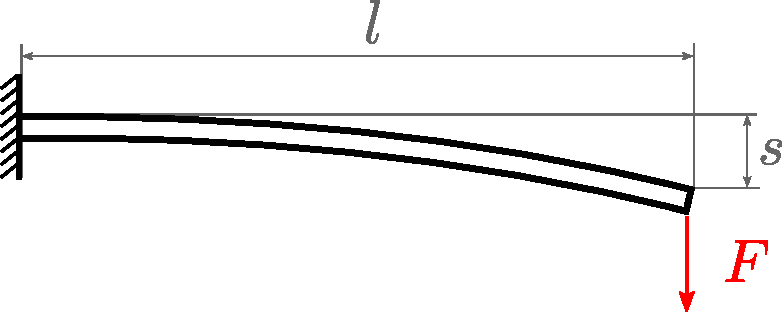
\includegraphics[width=0.5\textwidth]{figures/bending-test/setup.pdf}
\caption{Experimental setup}
\label{fig:bending-test}
\end{figure}

The elastic modulus can then be calculated depending on the cross section geometry using the equations in Table~\ref{tbl:bending-test}.

\begin{table}[H]
\centering
\begin{tabular}{| c | l |}
\hline
\textbf{Test geometry} & \textbf{Elastic Modulus} \\ \hline
\raisebox{-.5\height}{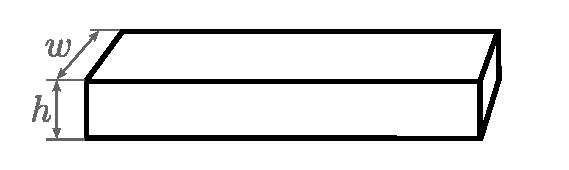
\includegraphics[width=0.4\textwidth]{figures/bending-test/sections-uniform.pdf}} & $\displaystyle E = \frac{4}{wh^3}\,\frac{Fl^3}{s}$ \\ \hline
\raisebox{-.5\height}{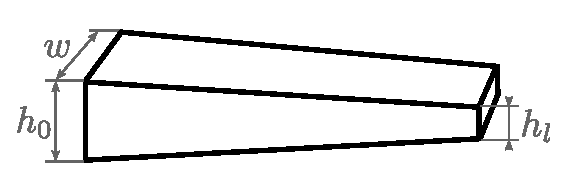
\includegraphics[width=0.4\textwidth]{figures/bending-test/sections-tapered.pdf}} & $\displaystyle E = \frac{12\,\ln(h_{l}\,l)+6}{w\,(h_{l}-h_{0})^3}\,\frac{Fl^3}{s}$ \\ \hline
\end{tabular}
\caption{Elastic modulus for different test geometries}
\label{tbl:bending-test}
\end{table}

\textbf{Note:} The following practical considerations might help with choosing a good test setup,

\begin{itemize}
\item The precision of the cross sections is very important, especially the height.
\item The equations above hold for slender beams and small deflections. The test setup should be chosen accordingly. As a rule of thumb: $h, s < l/15$.
\item A simple way to apply a defined force is to hang a mass $m$ onto the beam tip and use $F = m\cdot g$, with $g = \unit[9.81]{m/s^2}$.
\item If there is some small initial deflection due to gravity, then $s$ is simply the difference in deflection after application of the force.
\end{itemize}

\end{document}